\apendice{Especificación de diseño}

\section{Introducción}

En esta sección se van a detallar los diferentes diseños del software que se han desarrollado para implementar el proyecto.

\begin{itemize}
	\item Diseño de datos: En esta sección se explicará como están implementados los datos y clases desarrolladas tanto en la aplicación Android como en el proyecto de Eclipse.
	\item Diseño arquitectónico : En esta sección se explicará como están organizados los paquetes de los proyectos y como se interrelacionan entre sí.
	\item Diseño procedimental: En esta sección se explicarán los procedimientos más relevantes de la aplicación.
\end{itemize}

Para crear los diferentes diagramas requeridos en los diseños se han utilizado las herramientas \textit{Dia}\footnote{\url{http://dia-installer.de/index.html.es}} y \textit{Astah}\footnote{\url{http://astah.net/}}.

\section{Diseño de datos}

En esta sección se mostrará como están implementados los datos en la base de datos SQlite y a continuación, se mostrarán los diagramas de clases que detallan la estructura de datos seguida en ambos proyectos.

\subsection{Tablas de la base de datos}

Para guardar la información de las diferentes especies de setas de la aplicación se han creado las tablas de la figura \ref{figTablasSQlite}

\begin{figure}[h]
    \begin{center}%
        \begin{center}%
          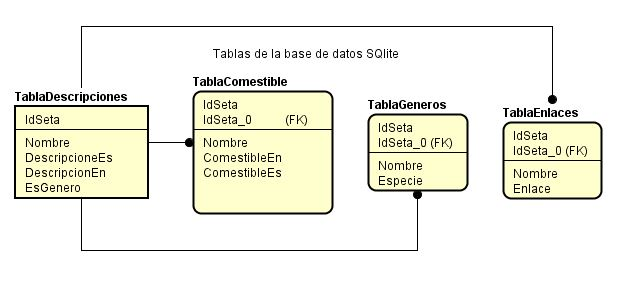
\includegraphics[width=1\textwidth]{imagenesAnexos/imagenesDiseno/TablasSQlite}%
          \caption{Tablas de la base de datos SQlite.}%
          \label{figTablasSQlite}%
        \end{center}%
  	\end{center}%
\end{figure}%

\begin{itemize}
	\item TablaComestible: Almacena la comestibilidad de una determinada especie en español e inglés.
	\item TablaDescripciones: Almacena la descripción de una determinada especie en español e inglés.
	\item TablaGeneros: Almacena el género al que pertenece una especie.
	\item TablaEnlaces: Almacena la url de la \textit{Wikipedia} de la especie. 
\end{itemize}

\subsection{Almacenamiento claves dicotómicas}

Las claves dicotómicas están guardadas en un archivo que contienen las siguientes estructuras java serializadas:

\begin{itemize}
	\item Map\textless String, ArrayList \textless String \textgreater \ \textgreater      arbolNodos : Este mapa contiene por cada género un arrayList con los siguientes tres mapas:
	\begin{itemize}
		\item Map\textless String, ArrayList\textless String\textgreater \ \textgreater arbolNodos: Mapa cuyas claves son los nodos y los valores son los nodos hijos de ese nodo padre. 
		
Este mapa nos sirve para contener la estructura de la clave.
		\item Map\textless String, ArrayList\textless String\textgreater \ \textgreater contenidoNodos: Mapa cuyas claves son los nodos y los valores son un array de Strings en el que la primera posición contienen la pregunta de ese nodo, la segunda posición es el enlace de esa especie, la tercera posición es el nodo padre y la cuarta posición contiene el género de esa especie.
		
Este mapa sirve para almacenar el contenido de cada nodo.
		\item Map\textless String, String\textgreater generosNodos: Mapa en el que las claves son géneros y los hijos son el nodo que contiene ese género dentro del mapa contenidoNodos.
		
Este mapa facilita acceder al nodo que contiene el género buscado de seta.
	\end{itemize}
\end{itemize}

\subsection{Diagramas de clases}
\subsubsection{Diagramas de clases del proyecto de Eclipse}

En la figura \ref{figDiagramaClasesJava} podemos observar las clases implementadas en el proyecto de Eclipse y que dependencias tienen entre sí. A continuación se muestra una breve descripción de la funcionalidad de cada clase y el paquete en el que esta contenida.

Para acceder a una descripción de los métodos acceder al \textbf{javadoc} de cada proyecto.

\begin{itemize}
	\item Paquete \textit{basedatossql}: Contiene las clases necesarias para crear y manejar la base de datos SQlite.
	\begin{itemize}
		\item Clase \textit{BDsql}: Clase que contiene los Métodos necesarios para acceder a una base de datos SQlite y manejarla.
		\item Clase \textit{CreadorBD}: Clase que crea la base de datos a partir de BDsql y DBpedia.
	\end{itemize}
	\item Paquete \textit{creador}: Contiene la clase que contiene el \textit{main} del proyecto.
	\begin{itemize}
		\item Clase \textit{CreadorBDyClaves}: Clase que lanza los métodos necesarios para crear la base de datos y extraer las claves dicotómicas.
	\end{itemize}
	\item Paquete \textit{dbpedia}: Contiene las clases necesarias para extraer la información de la DBpedia.
	\begin{itemize}
		\item Clase \textit{DBpedia}: Clase que contiene los métodos necesarios realizar consultas a la web semántica DBpedia.
	\end{itemize}
	\item Paquete \textit{traductor}: Contiene las clases necesarias para implementar un traductor automático.
	\begin{itemize}
		\item Clase \textit{Translator}: Clase que permite traducir cualquier texto a través de llamadas al traductor de Google. Clase descargada de \href{http://archana-testing.blogspot.com.es/2016/02/calling-google-translation-api-in-java.html}{\textit{archana-testing.}}
	\end{itemize}
	\item Paquete \textit{webscraping}: Contiene las clases necesarias realizar la extracción de las claves dicotómicas mediante técnicas de \textit{Web Scraping}.
	\begin{itemize}
		\item Clase \textit{ClaveDicotomica}: Clase que guarda la estructura de una clave dicotómica y tiene los métodos para cargarla de la url proporcionada y acceder a sus elementos. Esta preparada para funcionar con las claves de la página web \url{http://www.avelinosetas.info}
		\item Clase \textit{CreadorClaves}: Clase que contiene los métodos necesarios para serializar las claves dicotómicas.
	\end{itemize}
\end{itemize}
\begin{figure}[h]
    \begin{center}%
        \begin{center}%
          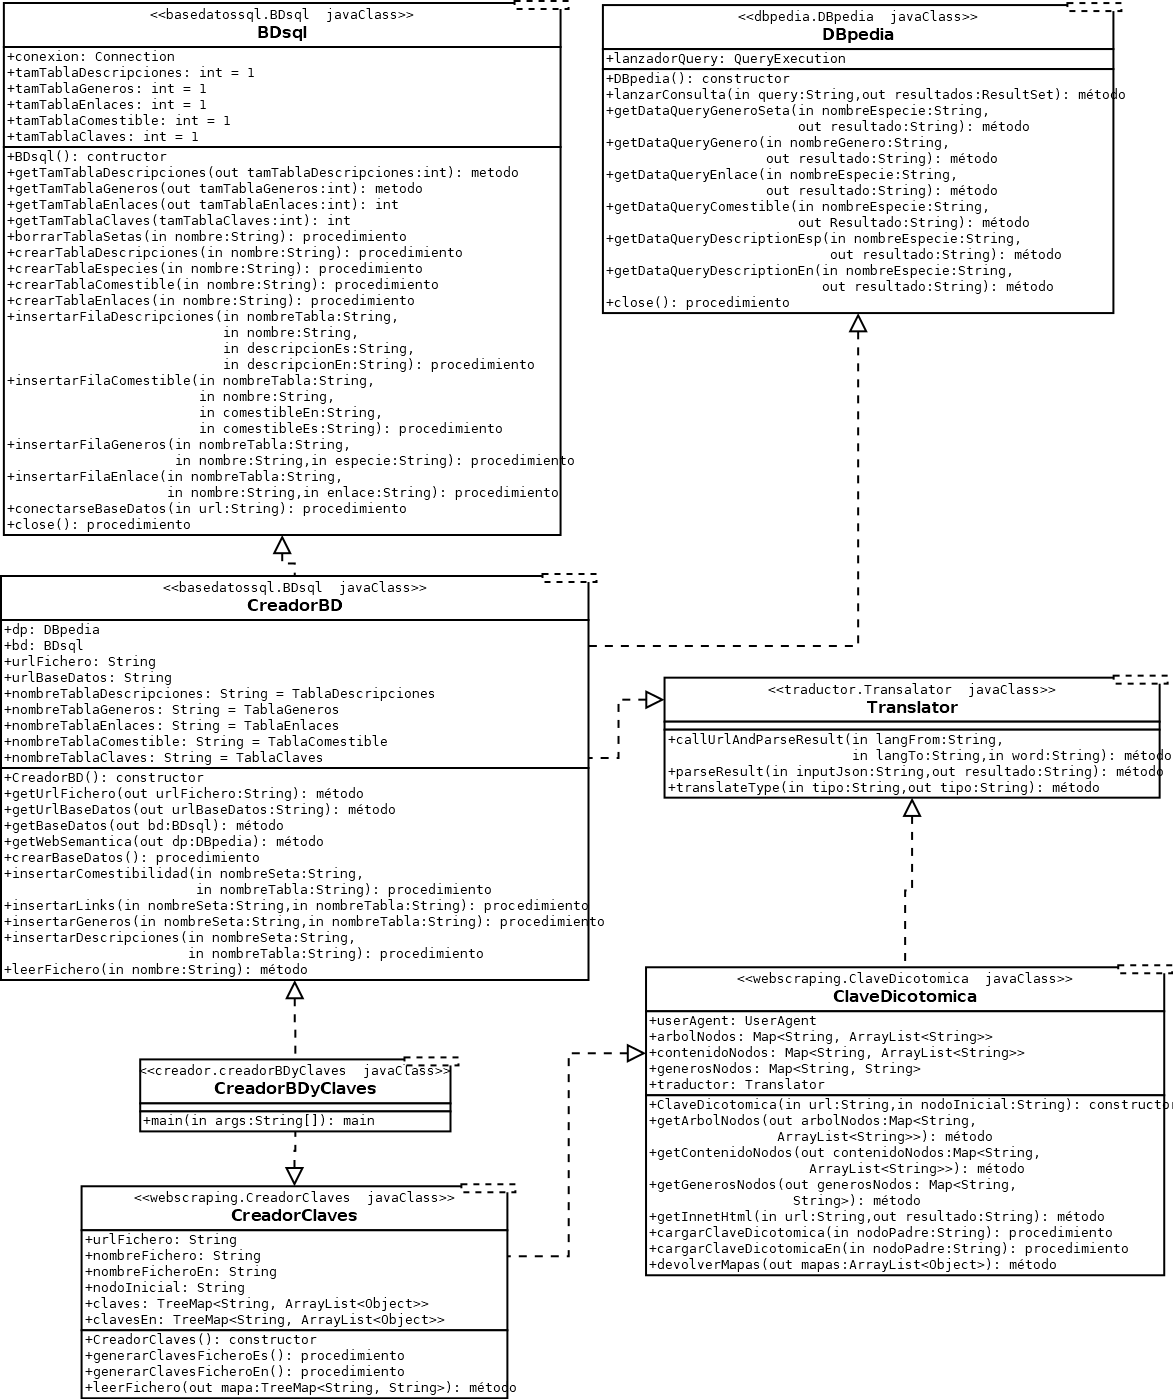
\includegraphics[width=1\textwidth]{imagenesAnexos/imagenesDiseno/DiagramaClasesJava}%
          \caption{Diagrama de clases del proyecto de Eclipse.}%
          \label{figDiagramaClasesJava}%
        \end{center}%
  	\end{center}%
\end{figure}%

\newpage
\subsubsection{Diagramas de clases del proyecto Android}

En esta sección se van a detallar los diagramas de clases del proyecto Android.

Para acceder a una descripción de los métodos acceder al \textbf{javadoc} de cada proyecto.

\begin{itemize}

	%1-PAQUETE BASEDATOS
	
	\item Paquete \textit{basedatos}: Paquete que contiene todas las clases necesarias para acceder a los datos de la aplicación. Diagrama de clases en la figura \ref{figDiagramaClasesAndroidBaseDatos}.
	\begin{itemize}
		\item Clase \textit{AccesoDatosExternos}: Clase que implementa las funciones necesarias para acceder a los datos externos a la aplicación que se encuentran en la carpeta assets.
		\item Clase \textit{DBsetas}: Clase que carga la base de datos SQLite encontrada en assets/databases.
		\item Clase \textit{DBsetasManager}: Clase que implementa los métodos para acceder y administrar la base de datos.
	\end{itemize}
	
	%2-PAQUETE CLASIFICADOR
	
	\item Paquete \textit{clasificador}: Paquete que contiene las clases y actividades relacionadas con la implementación y uso del clasificador de imágenes. Diagrama de clases en la figura \ref{figDiagramaClasesAndroidClasificador}.
	\begin{itemize}
		\item Clase \textit{RecogerFoto}: Clase que implementa la funcionalidad relacionada con la toma y guardado de fotografías.
		\item Clase \textit{TensorFlowImageClassifier}: Clase implementada por Tensorflow que permite usar un clasificador entrenado en Android.
	\end{itemize}
	
	%3-PAQUETE CLAVEDICOTOMICA
	
	\item Paquete \textit{clavedicotomica}: Paquete que contiene las clases relacionadas con mostrar las claves dicotómicas. Diagrama de clases en la figura \ref{figDiagramaClasesAndroidClaveDicotomica}.
	\begin{itemize}
		\item Clase \textit{ClaveDicotomica}: Clase que implementa la funcionalidad relacionada con mostrar la clave dicotómica seleccionada.
		\item Clase \textit{MostrarClaves}: Clase que muestra un listado de las claves dicotómicas de la aplicación.
	\end{itemize}
	
	%4-PAQUETE ELEGIRCLAVES
	
	\item Paquete \textit{elegirclaves}: Paquete que contiene las clases relacionadas con el filtrado de géneros de la clave general. Diagrama de clases en la figura \ref{figDiagramaClasesAndroidElegirClaves}.
	\begin{itemize}
		\item Clase \textit{AdaptadorSelector}: Clase que implementa el adaptador para cargar los elementos (ItemSelector) de la lista de géneros a seleccionar.
		\item Clase \textit{ViewHolderSelector}: Clase que implementa los elementos que se deben cargar en la lista (selector)y los relaciona con los elementos de la interfaz.
		\item Clase \textit{ElegirClaves}: Clase que muestra los géneros a elegir para filtrar la clave dicotómica general.
		\item Clase \textit{ItemSelector}: Clase que implementa los elementos del selector.
	\end{itemize}
	
	%5-PAQUETE INFORMACION
	
	\item Paquete \textit{informacion}: Paquete que contiene las clases relacionadas con mostrar la información de las distintas especies manejadas por la aplicación. Diagrama de clases en la figura \ref{figDiagramaClasesAndroidInformacion}.
	\begin{itemize}
		\item Clase \textit{MostrarSetas}: Clase que muestra las setas de la aplicación mediante un listado de tipo RecyclerView.
		\item Clase \textit{MostrarInformacionSetas}: Clase que muestra información relativa a la seta pulsada.
	\end{itemize}
	
	%6-PAQUETE LANZADOR
	
	\item Paquete \textit{lanzador}: Paquete que recoge la clase lanzadora de la aplicación. Diagrama de clases en la figura \ref{figDiagramaClasesAndroidLanzador}.
	\begin{itemize}
		\item Clase \textit{Lanzadora}: Clase que arranca la aplicación. Muestra los botones principales para acceder a las funcionalidades más importantes de la aplicación.
	\end{itemize}
	
	%7-PAQUETE RESULTADOS
	
	\item Paquete \textit{resultados}: Paquete que contiene las clases relacionadas con mostrar los resultados obtenidos por el clasificador. Diagrama de clases en la figura \ref{figDiagramaClasesAndroidResultados}.
	\begin{itemize}
		\item Clase \textit{AdaptadorSetasLista}:Clase que sirve de adaptador al sistema para cargar en cada elemento de la lista una foto y el nombre de la especie de la seta.
		\item Clase \textit{SetasListaHolder}: Clase que contiene cada par imagenView-TextView de cada elemento de la lista.
		\item Clase \textit{SetasLista}: Clase que implementa el contenido que va a tener la lista de imágenes que se muestran como resultado tras clasificar una foto.
		\item Clase \textit{MostrarComparativa}: Clase que muestra la foto introducida por el usuario y la seleccionada.
		\item Clase \textit{MostrarResultados}: Clase que implementa la funcionalidad de la actividad que muestra los resultados obtenidos tras
clasificar una foto.
	\end{itemize}
	
	%8-PAQUETE TARJETASCLAVES
	
	\item Paquete \textit{tarjetasclaves}: Paquete que contiene las clases relacionadas con mostrar el listado de claves dicotómicas disponibles en la aplicación. Diagrama de clases en la figura \ref{figDiagramaClasesAndroidTarjetasClaves}.
	\begin{itemize}
		\item Clase \textit{AdaptadorTarjetasClaves}: Clase que implementa el adaptador para cargar los elementos de la lista de las claves dicotómicas.
		\item Clase \textit{ViewHolder}: Clase que implementa los elementos que se deben cargar en la lista de claves.
		\item Clase \textit{TarjetaClave}: Clase que implementa el contenido de una tarjeta de claves dicotómicas.
	\end{itemize}
	
	%9-PAQUETE TARJETASCLAVES
	
	\item Paquete \textit{tarjetassetas}: Paquete que contiene las clases relacionadas con mostrar el listado de especies disponibles en la aplicación. Diagrama de clases en la figura \ref{figDiagramaClasesAndroidTarjetasSetas}.
	\begin{itemize}
		\item Clase \textit{AdaptadorTarjetasSetas}: Clase que implementa el adaptador para cargar los elementos de la lista de setas.
		\item Clase \textit{ViewHolder}: Clase que implementa los elementos que se deben cargar en la lista de setas.
		\item Clase \textit{TarjetaSeta}: Clase que implementa el contenido de una tarjeta de la lista de especies de setas.
	\end{itemize}
	
\end{itemize}

\newpage
%1
\begin{figure}[h]
    \begin{center}%
        \begin{center}%
          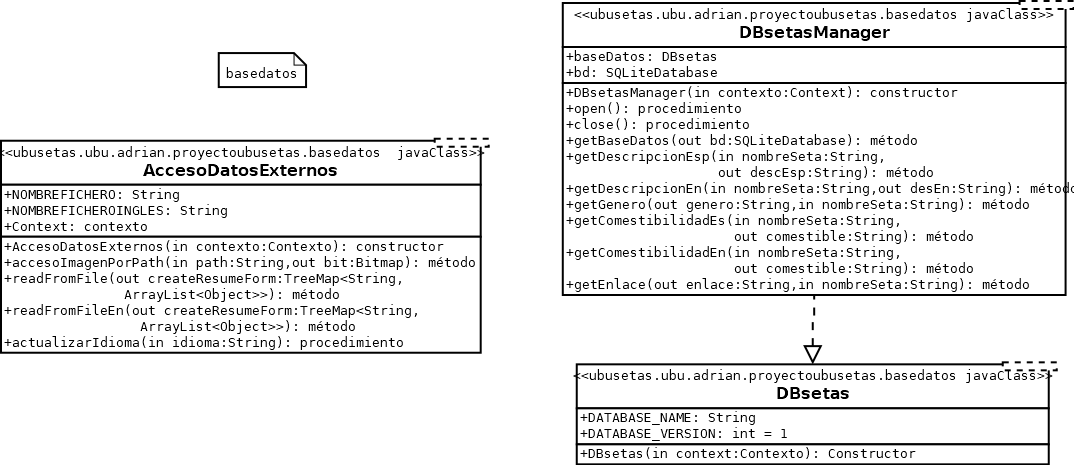
\includegraphics[width=1\textwidth]{imagenesAnexos/imagenesDiseno/DiagramaClasesAndroidBaseDatos}%
          \caption{Diagrama de clases del paquete basedatos.}%
          \label{figDiagramaClasesAndroidBaseDatos}%
        \end{center}%
  	\end{center}%
\end{figure}%
%2
\begin{figure}[h]
    \begin{center}%
        \begin{center}%
          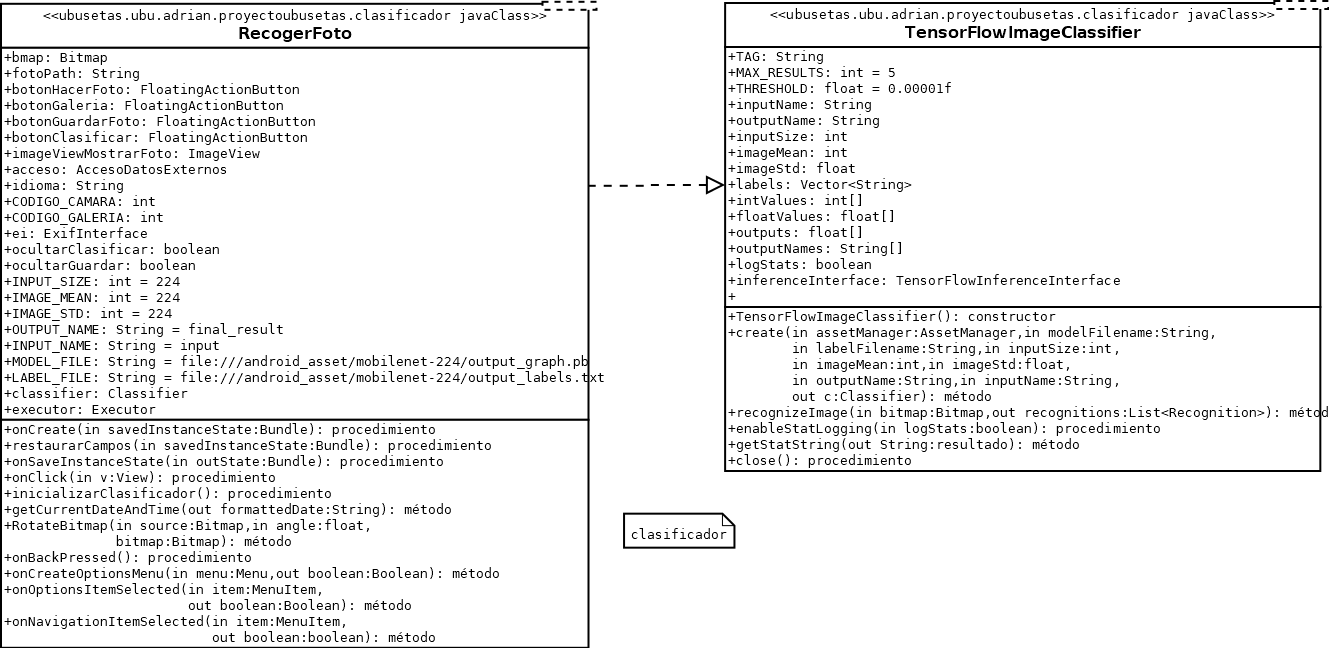
\includegraphics[width=1\textwidth]{imagenesAnexos/imagenesDiseno/DiagramaClasesAndroidClasificador}%
          \caption{Diagrama de clases del paquete clasificador.}%
          \label{figDiagramaClasesAndroidClasificador}%
        \end{center}%
  	\end{center}%
\end{figure}%
%3
\begin{figure}[h]
    \begin{center}%
        \begin{center}%
          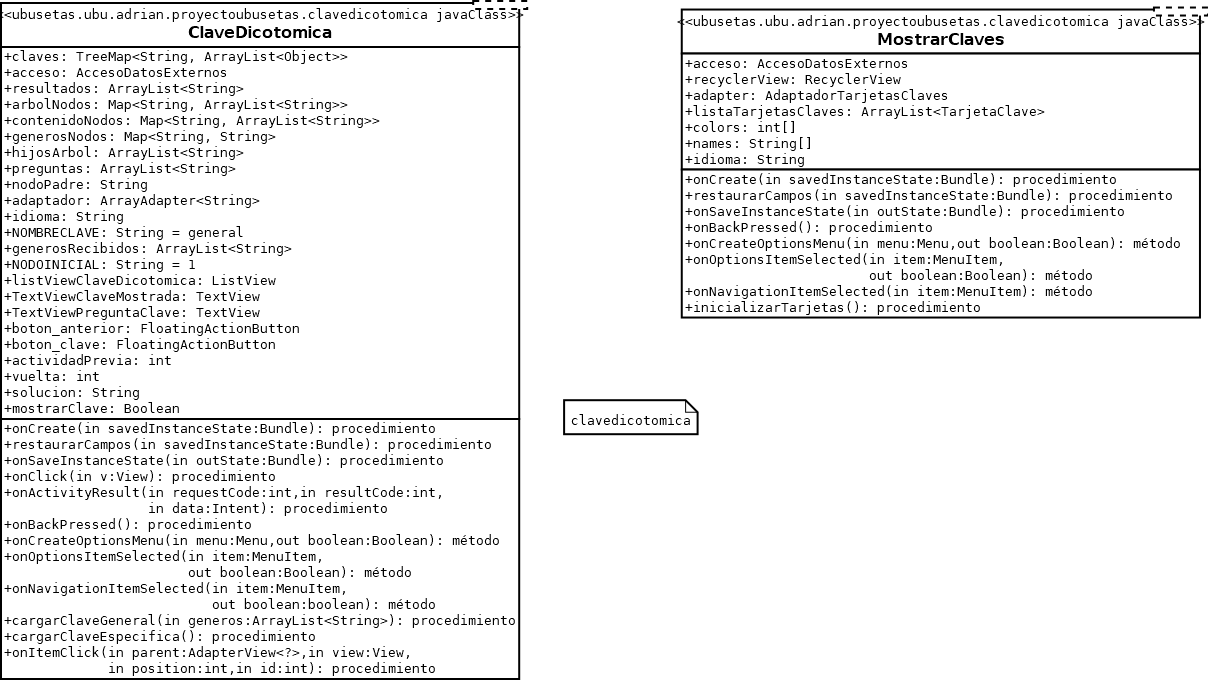
\includegraphics[width=1\textwidth]{imagenesAnexos/imagenesDiseno/DiagramaClasesAndroidClaveDicotomica}%
          \caption{Diagrama de clases del paquete clavedicotomica.}%
          \label{figDiagramaClasesAndroidClaveDicotomica}%
        \end{center}%
  	\end{center}%
\end{figure}%
%4
\begin{figure}[h]
    \begin{center}%
        \begin{center}%
          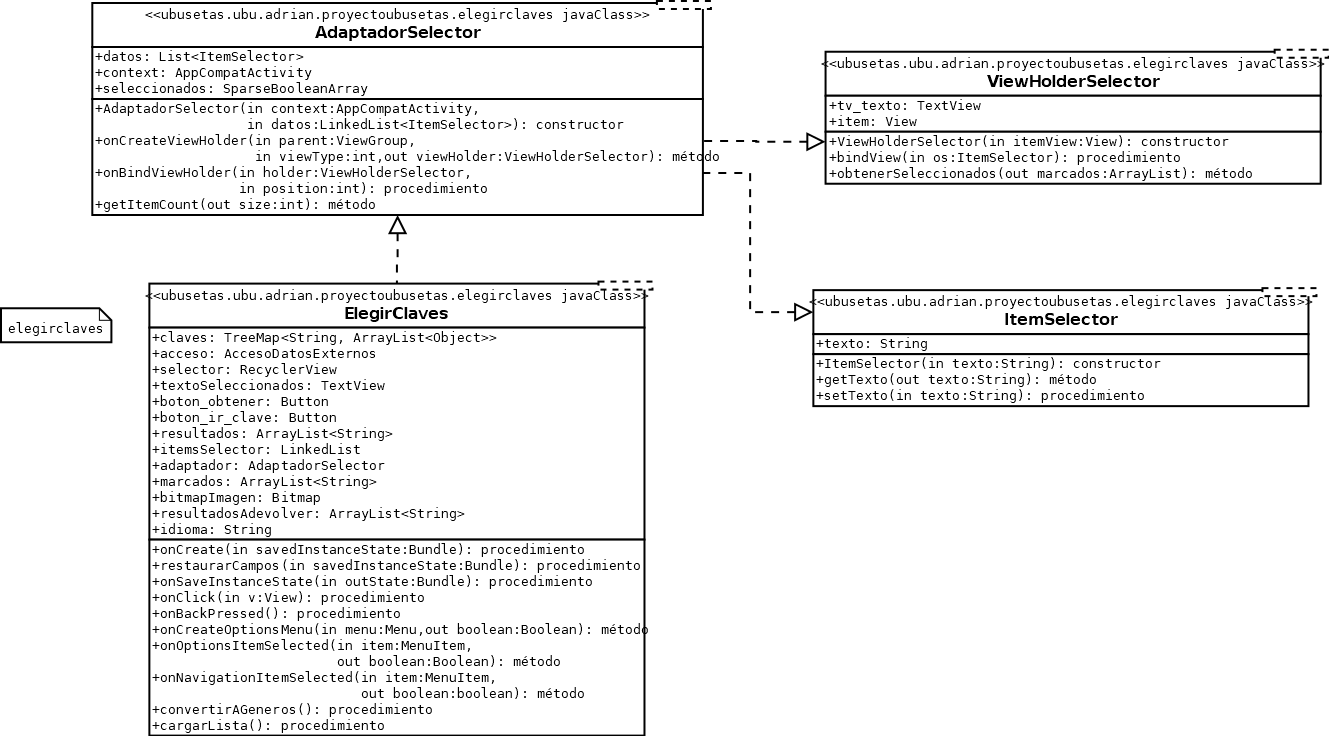
\includegraphics[width=1\textwidth]{imagenesAnexos/imagenesDiseno/DiagramaClasesAndroidElegirClaves}%
          \caption{Diagrama de clases del paquete elegirclaves.}%
          \label{figDiagramaClasesAndroidElegirClaves}%
        \end{center}%
  	\end{center}%
\end{figure}%
%5
\begin{figure}[h]
    \begin{center}%
        \begin{center}%
          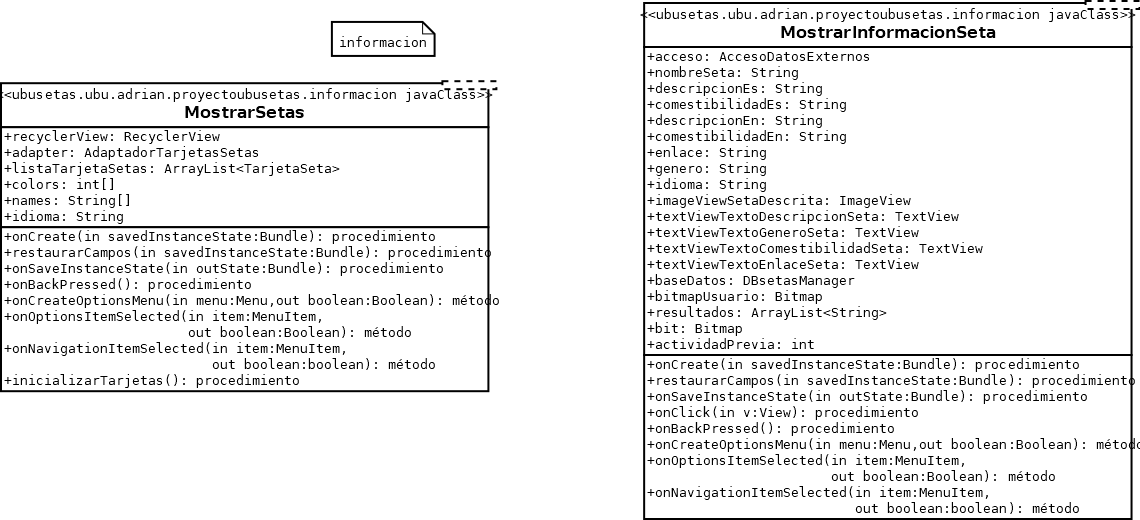
\includegraphics[width=1\textwidth]{imagenesAnexos/imagenesDiseno/DiagramaClasesAndroidInformacion}%
          \caption{Diagrama de clases del paquete informacion.}%
          \label{figDiagramaClasesAndroidInformacion}%
        \end{center}%
  	\end{center}%
\end{figure}%
%6
\begin{figure}[h]
    \begin{center}%
        \begin{center}%
          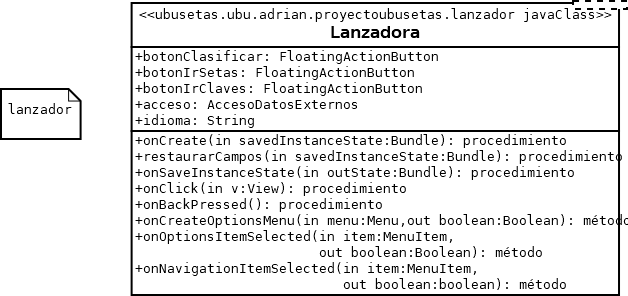
\includegraphics[width=1\textwidth]{imagenesAnexos/imagenesDiseno/DiagramaClasesAndroidLanzador}%
          \caption{Diagrama de clases del paquete lanzador.}%
          \label{figDiagramaClasesAndroidLanzador}%
        \end{center}%
  	\end{center}%
\end{figure}%
%7
\begin{figure}[h]
    \begin{center}%
        \begin{center}%
          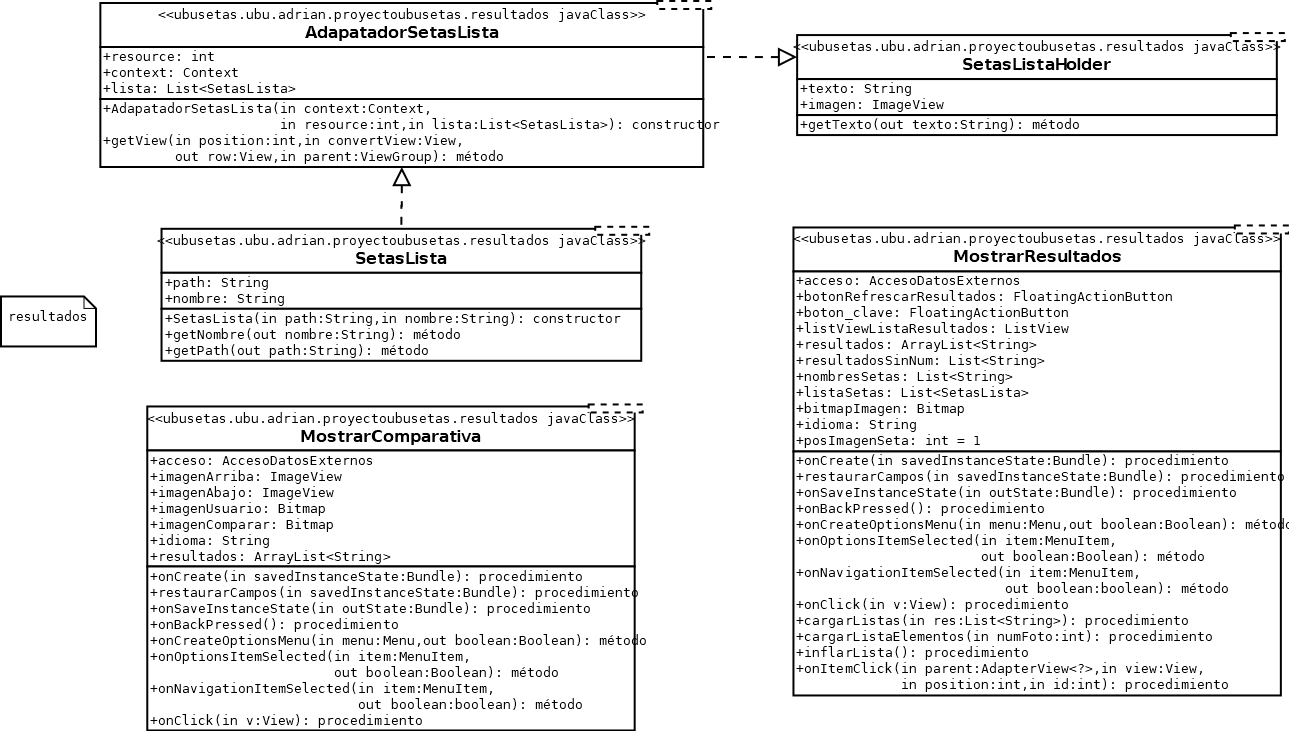
\includegraphics[width=1\textwidth]{imagenesAnexos/imagenesDiseno/DiagramaClasesAndroidResultados}%
          \caption{Diagrama de clases del paquete resultados.}%
          \label{figDiagramaClasesAndroidResultados}%
        \end{center}%
  	\end{center}%
\end{figure}%
%8
\begin{figure}[h]
    \begin{center}%
        \begin{center}%
          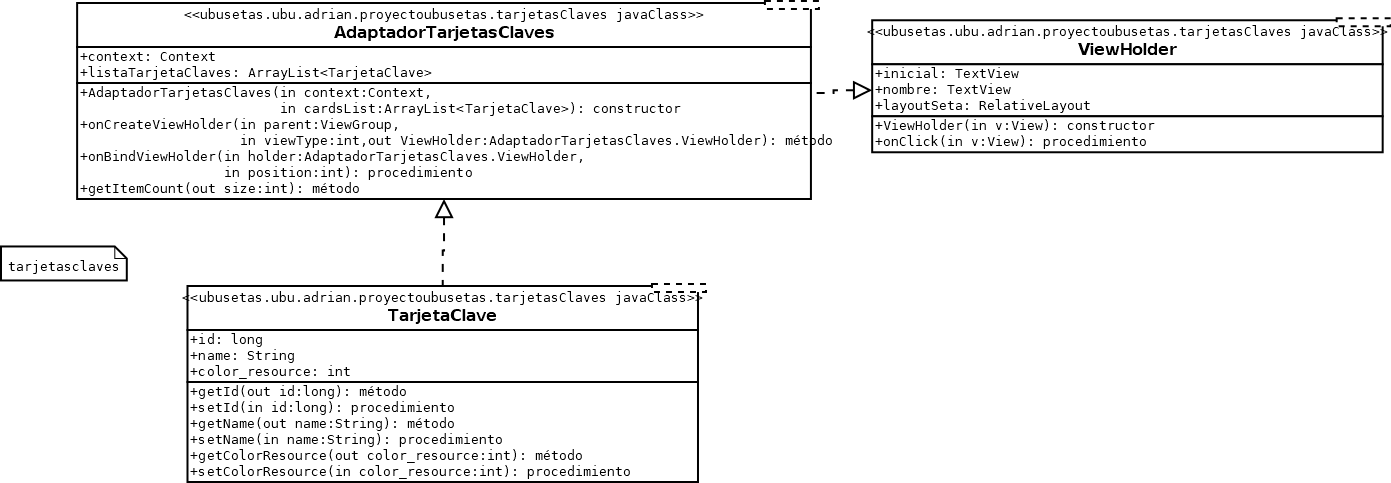
\includegraphics[width=1\textwidth]{imagenesAnexos/imagenesDiseno/DiagramaClasesAndroidTarjetasClaves}%
          \caption{Diagrama de clases del paquete tarjetasclaves.}%
          \label{figDiagramaClasesAndroidTarjetasClaves}%
        \end{center}%
  	\end{center}%
\end{figure}%
%9

\begin{figure}[h]
    \begin{center}%
        \begin{center}%
          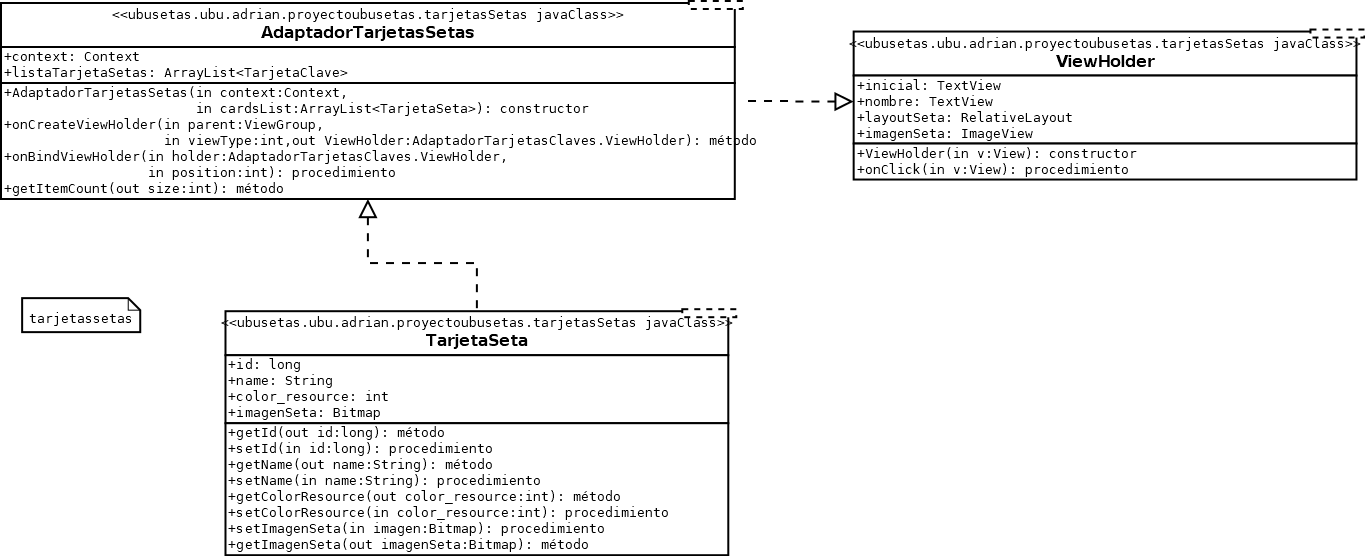
\includegraphics[width=1\textwidth]{imagenesAnexos/imagenesDiseno/DiagramaClasesAndroidTarjetasSetas}%
          \caption{Diagrama de clases del paquete tarjetassetas.}%
          \label{figDiagramaClasesAndroidTarjetasSetas}%
        \end{center}%
  	\end{center}%
\end{figure}%

\clearpage

\section{Diseño procedimental} \label{disenoProcedimental}

Sección en la que se van a explicar los pasos para realizar los procesos más relevantes de la aplicación Android.

\subsection{Clasificar imagen}

Para clasificar una imagen desde la aplicación Andrroi, el usuario deberá seguir estos pasos:

\begin{itemize}
	\item Paso 1: Iniciar la aplicación.
	\item Paso 2: Pulsar sobre el botón de \textit{clasificar} disponible en la actividad lanzadora o en el menú.
	\item Paso 3: Pulsar sobre el botón de galería o cámara disponibles en la siguiente actividad para cargar la imagen, bien desde la galería o desde la cámara de fotos del móvil.
	\item Paso 4: Introducir una imagen de una seta.
	\item Paso 5: En este momento, aparecerá el botón de clasificar. Pulsar sobre este botón.
	\item Paso 6: La aplicación mostrará un listado de las especies más probables clasificadas para esa imagen.
\end{itemize}

\subsection{Selección de géneros para usar la clave dicotómica}

Una vez el usuario haya clasificado una imagen, podrá acceder a una clave dicotómica filtrada según los resultados obtenidos. El usuario podrá elegir los géneros de setas sobre los que aplicar la clave, si lo desea podrá aplicarla sobre todos los disponibles.

\begin{itemize}
	\item Paso 1: Realizar los pasos del procedimiento \textit{Clasificar imagen}.
	\item Paso 2: Pulsar sobre el botón de acceso a la clave dicotómica.
	\item Paso 3: Seleccionar de la lista los géneros deseados. Para ello primero se eligen los géneros pulsando sobre ellos y después se pulsa sobre el botón de seleccionar.
	\item Paso 4: Pulsar sobre el botón \textit{ir clave dicotómica}.
	\item Paso 5: En este momento, se mostrarán las preguntas relacionadas con los géneros seleccionados.
\end{itemize}

\subsection{Seleccionar clave dicotómica}

El usuario podrá seleccionar una clave de las disponibles en la aplicación.

\begin{itemize}
	\item Paso 1: Iniciar la aplicación.
	\item Paso 2: Pulsar sobre el botón de \textit{ir claves} disponible en la actividad lanzadora o en el menú.
	\item Paso 3: Pulsar sobre la clave dicotómica del género de seta deseado.
	\item Paso 4: En este momento, se mostrarán las preguntas relacionadas con la clave seleccionada.
\end{itemize}
\subsection{Acceder a información de especie de seta}

El usuario podrá acceder a la información de una especie de seta recogida por la aplicación. Esta acción se podrá realizar de las siguientes dos formas:

\subsubsection{Forma 1}

\begin{itemize}
	\item Paso 1: Iniciar la aplicación.
	\item Paso 2: Pulsar sobre el botón de \textit{mostrar setas} disponible en la actividad lanzadora o en el menú.
	\item Paso 3: Pulsar sobre la especie de seta deseada.
	\item Paso 4: En este momento, se mostrará información describiendo la especie pulsada.
\end{itemize}

\subsubsection{Forma 2}

\begin{itemize}
	\item Paso 1: Realizar los pasos del procedimiento \textit{Clasificar imagen}.
	\item Paso 2: Mantener pulsado uno de los resultados
	\item Paso 3: En este momento, se mostrará información describiendo la especie pulsada.
\end{itemize}

\subsection{Responder una clave dicotómica}

El usuario podrá responder las preguntas de la clave dicotómica. Esta acción se podrá realizar de las siguientes dos formas:

\subsubsection{Forma 1}

\begin{itemize}
	\item Paso 1: Realizar los pasos del procedimiento \textit{Seleccionar clave dicotómica}.
	\item Paso 2: Ir respondiendo a las preguntas que va realizando la aplicación.
	\item Paso 3: El usuario podrá volver a la pregunta anterior pulsando el botón de volver.
	\item Paso 4: Una vez se hayan respondido todas las preguntas, se mostrará el género o especie clasificado por la clave, según esta sea la clave de géneros o una de especies.
	\item Paso 5: Si la aplicación tiene una clave dicotómica del género clasificado, se notificará al usuario y aparecerá un botón que le redirija a la clave que discrimina las especies de ese género.
\end{itemize}

\subsubsection{Forma 2}

\begin{itemize}
	\item Paso 1: Realizar los pasos del procedimiento \textit{Selección de géneros para usar la clave dicotómica}.
	\item Paso 2: Ir respondiendo a las preguntas que va realizando la aplicación.
	\item Paso 3: El usuario podrá volver a la pregunta anterior pulsando el botón de volver.
	\item Paso 4: Una vez se hayan respondido todas las preguntas, se mostrará el género clasificado por la clave
	\item Paso 5: Si la aplicación tiene una clave dicotómica del género clasificado, se notificará al usuario y aparecerá un botón que le redirija a la clave que discrimina las especies de ese género.
\end{itemize}

\section{Diseño arquitectónico}

En esta sección se va a mostrar la estructura de paquetes seguida tanto en el proyecto Android como en el de Eclipse.

\subsection{Proyecto Eclipse}

A continuación se muestra una descripción de los paquetes del proyecto de Eclipse y como se relacionan entre sí.

\begin{itemize}
	\item Paquete \textit{basedatossql}: Contiene las clases necesarias para crear y manejar la base de datos SQlite.
	\item Paquete \textit{creador}: Contiene la clase que contiene el \textit{main} del proyecto. Hace uso de los paquetes dbpedia y webscraping para extraer toda la información necesaria por la aplicación.
	\item Paquete \textit{dbpedia}: Contiene las clases necesarias para extraer la información de la DBpedia. Hace uso del paquete traductor para traducir al inglés la información. Hace uso del paquete basededatossql para almacenar la información consultada en la base de datos.
	\item Paquete \textit{traductor}: Contiene las clases necesarias para implementar un traductor automático.
	\item Paquete \textit{webscraping}: Contiene las clases necesarias realizar la extracción de las claves dicotómicas mediante técnicas de \textit{Web Scraping}.Hace uso del paquete traductor para traducir las claves dicotómicas.
\end{itemize}

En la figura \ref{figDiagramaPaquetesJava} se muestra el diagrama de paquetes del proyecto de Eclipse.

\begin{figure}[h]
    \begin{center}%
        \begin{center}%
          \includegraphics[width=1\textwidth]{imagenesAnexos/imagenesDiseno/DiagramaPaquetesJava}%
          \caption{Diagrama de paquetes del proyecto de Eclipse.}%
          \label{figDiagramaPaquetesJava}%
        \end{center}%
  	\end{center}%
\end{figure}%

\newpage
\subsection{Proyecto Android}

A continuación se muestra una descripción de los paquetes del proyecto Android y como se relacionan entre sí.

\begin{itemize}

	%1-PAQUETE BASEDATOS
	
	\item Paquete \textit{basedatos}: Paquete que contiene todas las clases necesarias para acceder a los datos de la aplicación.
	
	%2-PAQUETE CLASIFICADOR
	
	\item Paquete \textit{clasificador}: Paquete que contiene las clases y actividades relacionadas con la implementación y uso del clasificador de imágenes.
	
	%3-PAQUETE CLAVEDICOTOMICA
	
	\item Paquete \textit{clavedicotomica}: Paquete que contiene las clases relacionadas con mostrar las claves dicotómicas. Hace uso del paquete base de datos para extraer las claves dicotómicas del fichero serializado. Usa el paquete tarjetasclaves para implementar el listado de claves.
	
	%4-PAQUETE ELEGIRCLAVES
	
	\item Paquete \textit{elegirclaves}: Paquete que contiene las clases relacionadas con el filtrado de géneros de la clave general. 
	
	%5-PAQUETE INFORMACION
	
	\item Paquete \textit{informacion}: Paquete que contiene las clases relacionadas con mostrar la información de las distintas especies manejadas por la aplicación. Hace uso del paquete basedatos para extraer la información de la base de datos SQlite y acceder a las imágenes de las setas, situadas en los directorios externos. Usa el paquete tarjetassetas para implementar el listado de especies de setas.
	
	%6-PAQUETE LANZADOR
	
	\item Paquete \textit{lanzador}: Paquete que recoje la clase lanzadora de la aplicación.
	
	%7-PAQUETE RESULTADOS
	
	\item Paquete \textit{resultados}: Paquete que contiene las clases relacionadas con mostrar los resultados obtenidos por el clasificador. Hace uso del paquete basedatos para acceder a las imágenes de las setas, situadas en los directorios externos.
	
	%8-PAQUETE TARJETASCLAVES
	
	\item Paquete \textit{tarjetasclaves}: Paquete que contiene las clases relacionadas con mostrar el listado de claves dicotómicas disponibles en la aplicación.
	
	%9-PAQUETE TARJETASCLAVES
	
	\item Paquete \textit{tarjetassetas}: Paquete que contiene las clases relacionadas con mostrar el listado de especies disponibles en la aplicación.
	
\end{itemize}

En la figura \ref{figDiagramaPaquetesAndroid} se muestra el diagrama de paquetes del proyecto Android. 
\begin{figure}[h]
    \begin{center}%
        \begin{center}%
          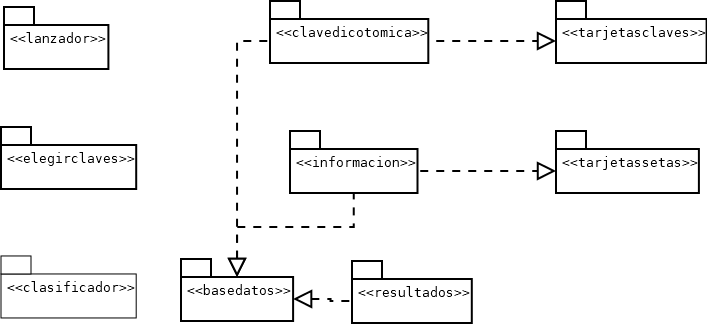
\includegraphics[width=1\textwidth]{imagenesAnexos/imagenesDiseno/DiagramaPaquetesAndroid}%
          \caption{Diagrama de paquetes del proyecto Android.}%
          \label{figDiagramaPaquetesAndroid}%
        \end{center}%
  	\end{center}%
\end{figure}%

\section{Diseño de la interfaz}

En esta sección se van a mostrar los prototipos que se realizaron para diseñar la interfaz y un ejemplo de como es la interfaz final de la aplicación Android.

\subsection{Prototipado}

El prototipado de la aplicación se realizó de manera manual, dibujando un diseño inicial de lo que iba a ser la interfaz de cada actividad. En estas tarjetas se dibujo el diseño con y sin menú, así como la vista horizontal y vertical de la aplicación. A continuación se muestran las tarjetas de las diferentes actividades.

\begin{itemize}

	%0-ACTIVIDAD LANZADORA
	
	\item Actividad Lanzadora \ref{figActividadLanzadora0}:
	\begin{figure}[h]
    	\begin{center}%
        	\begin{center}%
          	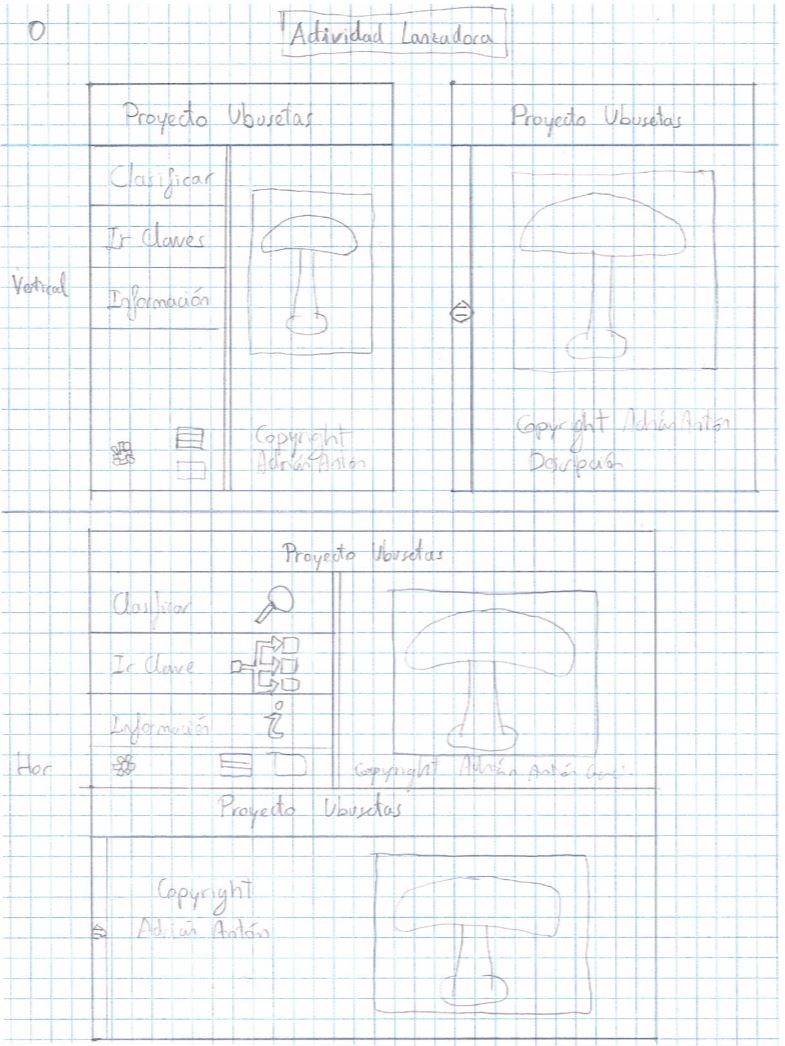
\includegraphics[width=0.6\textwidth]{imagenesAnexos/prototipado/ActividadLanzadora0}%
          	\caption{Prototipo actividad Lanzadora.}%
          	\label{figActividadLanzadora0}%
        	\end{center}%
  		\end{center}%
	\end{figure}%
	\clearpage
		%1-ACTIVIDAD RECOGER FOTO
	
	\item Actividad Recoger Foto \ref{figActividadRecogerFoto1}:
	\begin{figure}[h]
    	\begin{center}%
        	\begin{center}%
          	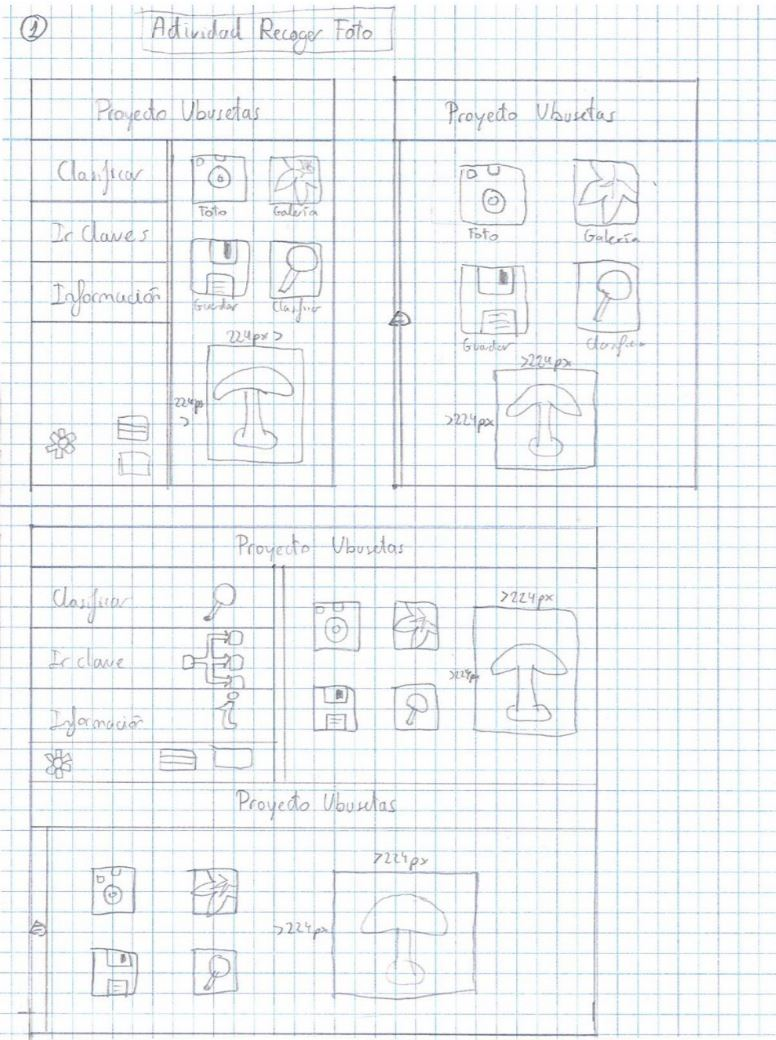
\includegraphics[width=0.8\textwidth]{imagenesAnexos/prototipado/ActividadRecogerFoto1}%
          	\caption{Prototipo actividad Recoger Foto.}%
          	\label{figActividadRecogerFoto1}%
        	\end{center}%
  		\end{center}%
	\end{figure}%
	\clearpage
		%2-ACTIVIDAD MOSTRAR CLAVES
	
	\item Actividad Mostrar Claves \ref{figActividadMostrarClaves2}:
	\begin{figure}[h]
    	\begin{center}%
        	\begin{center}%
          	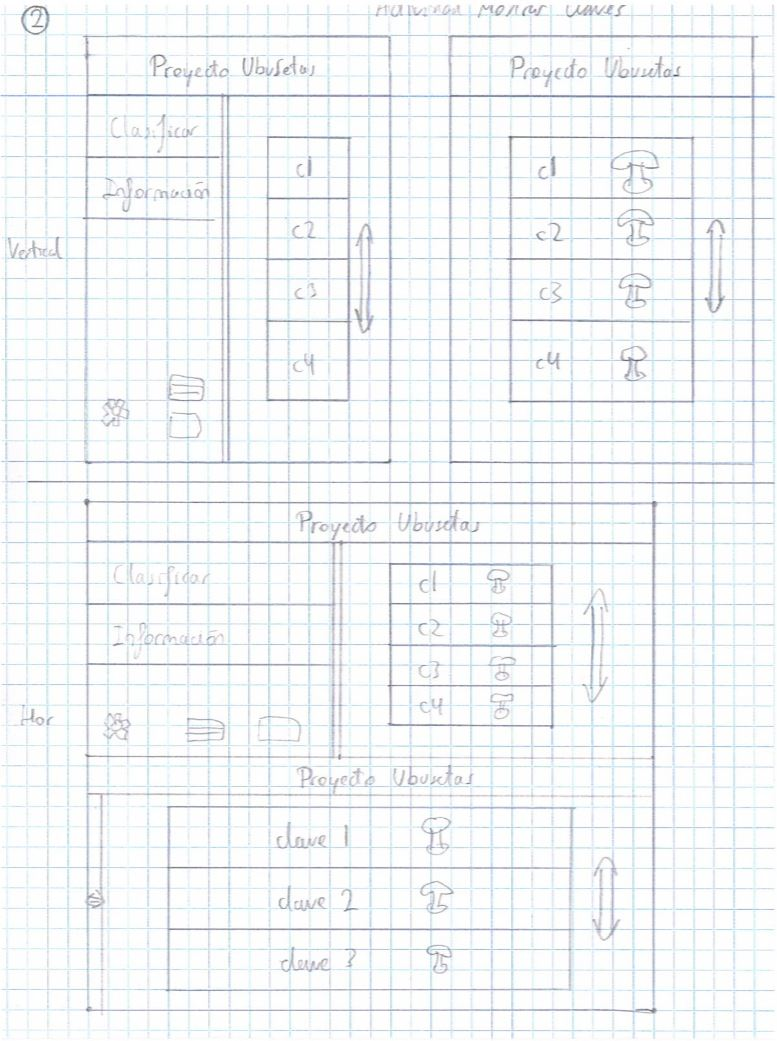
\includegraphics[width=0.8\textwidth]{imagenesAnexos/prototipado/ActividadMostrarClaves2}%
          	\caption{Prototipo actividad Mostrar Claves.}%
          	\label{figActividadMostrarClaves2}%
        	\end{center}%
  		\end{center}%
	\end{figure}%
	\clearpage
	
		%3-ACTIVIDAD MOSTRAR SETAS
	
	\item Actividad Mostrar Setas\ref{figActividadMostrarSetas3}:
	\begin{figure}[h]
    	\begin{center}%
        	\begin{center}%
          	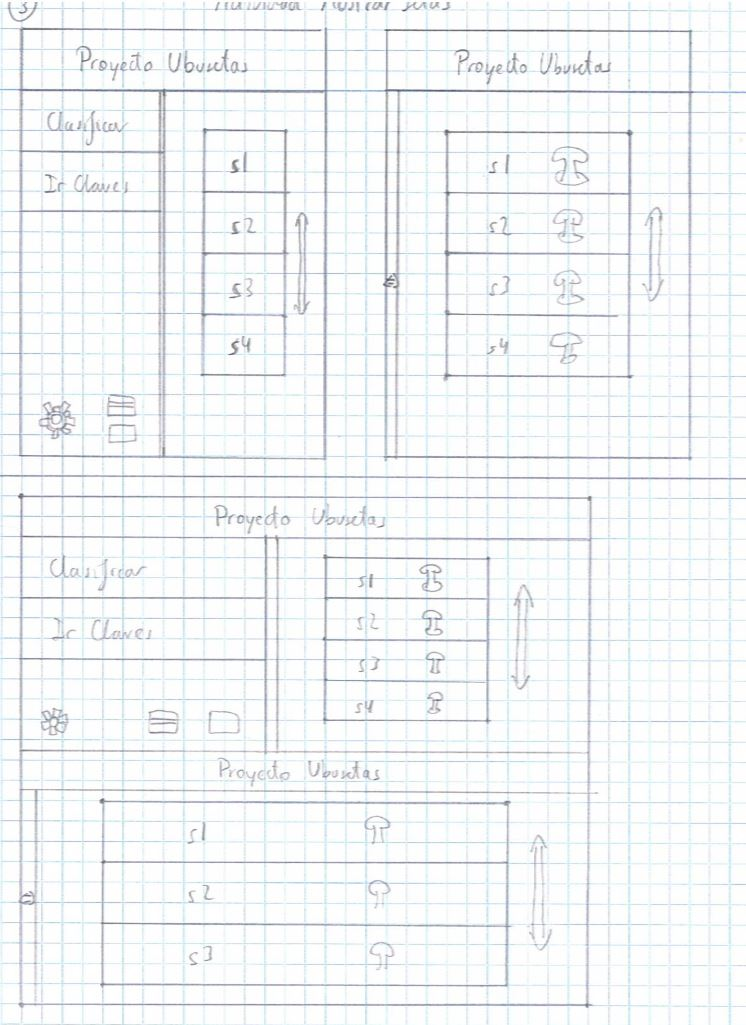
\includegraphics[width=0.8\textwidth]{imagenesAnexos/prototipado/ActividadMostrarSetas3}%
          	\caption{Prototipo actividad Mostrar Setas.}%
          	\label{figActividadMostrarSetas3}%
        	\end{center}%
  		\end{center}%
	\end{figure}%
	\clearpage
	
		%4-ACTIVIDAD MOSTRAR RESULTADOS
	
	\item Actividad Mostrar Resultados \ref{figActividadMostrarResultados4}:
	\begin{figure}[h]
    	\begin{center}%
        	\begin{center}%
          	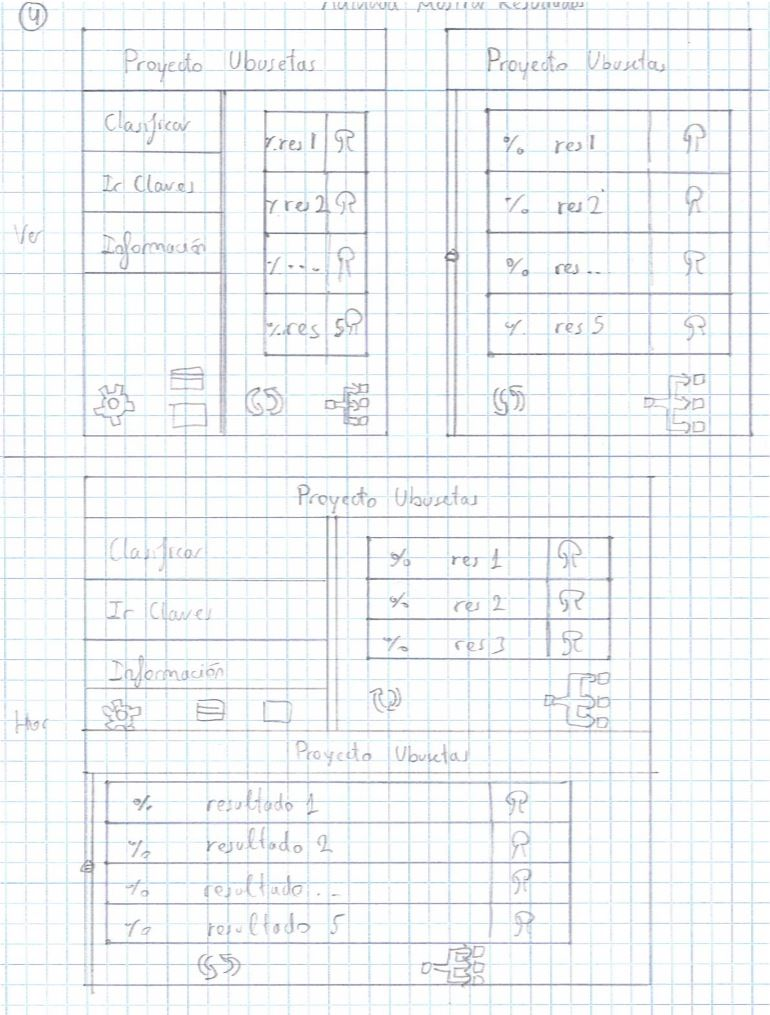
\includegraphics[width=0.8\textwidth]{imagenesAnexos/prototipado/ActividadMostrarResultados4}%
          	\caption{Prototipo actividad Mostrar Resultados.}%
          	\label{figActividadMostrarResultados4}%
        	\end{center}%
  		\end{center}%
	\end{figure}%
	\clearpage
	
		%5-ACTIVIDAD CLAVE DICOTOMICA
	
	\item Actividad Clave Dicotómica \ref{figActividadClaveDicotomica5}:
	\begin{figure}[h]
    	\begin{center}%
        	\begin{center}%
          	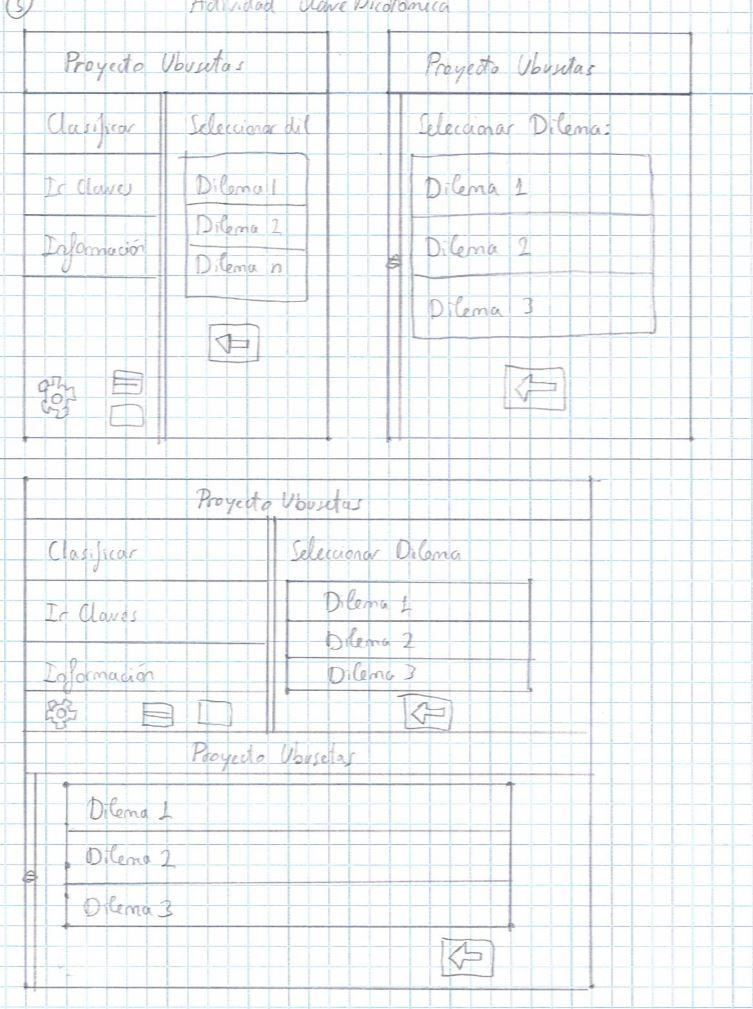
\includegraphics[width=0.8\textwidth]{imagenesAnexos/prototipado/ActividadClaveDicotomica5}%
          	\caption{Prototipo actividad Clave Dicotómica.}%
          	\label{figActividadClaveDicotomica5}%
        	\end{center}%
  		\end{center}%
	\end{figure}%
	\clearpage
	
		%6-ACTIVIDAD MOSTRAR INFORMACIÓN
	
	\item Actividad Mostrar Información \ref{figActividadMostrarInformacion6}:
	\begin{figure}[h]
    	\begin{center}%
        	\begin{center}%
          	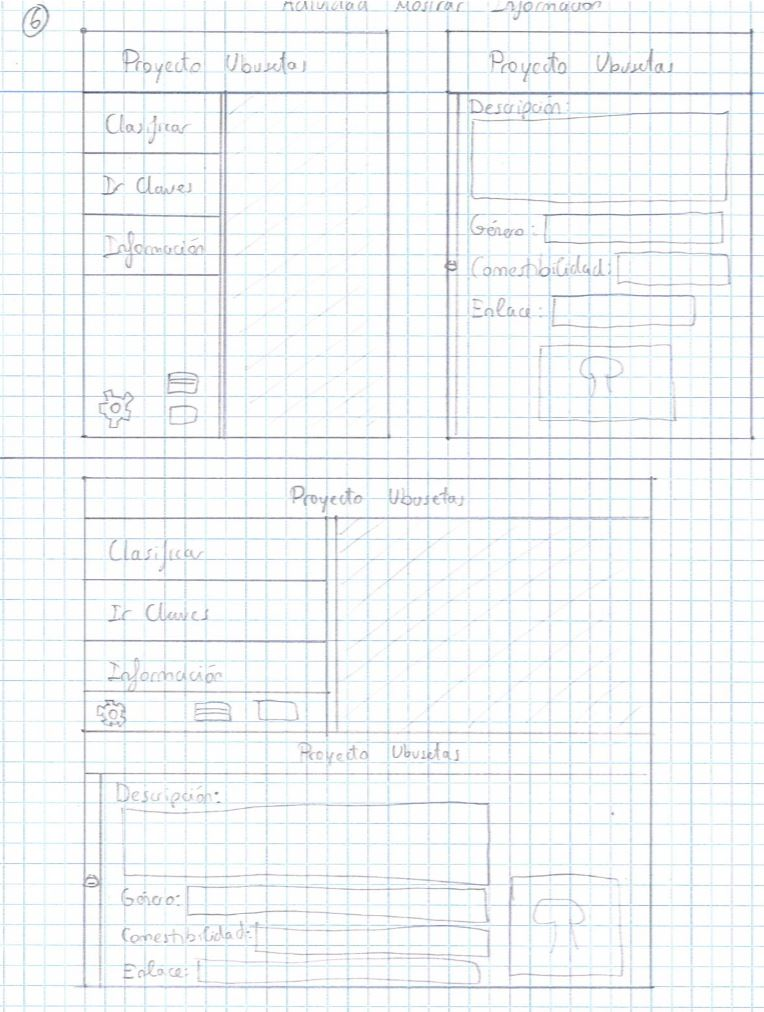
\includegraphics[width=0.8\textwidth]{imagenesAnexos/prototipado/ActividadMostrarInformacion6}%
          	\caption{Prototipo Mostrar Información.}%
          	\label{figActividadMostrarInformacion6}%
        	\end{center}%
  		\end{center}%
	\end{figure}%
	\clearpage
	
		%7-ACTIVIDAD ELEGIR CLAVES
	
	\item Actividad Elegir Claves \ref{figActividadElegirClaves7}:
	\begin{figure}[h]
    	\begin{center}%
        	\begin{center}%
          	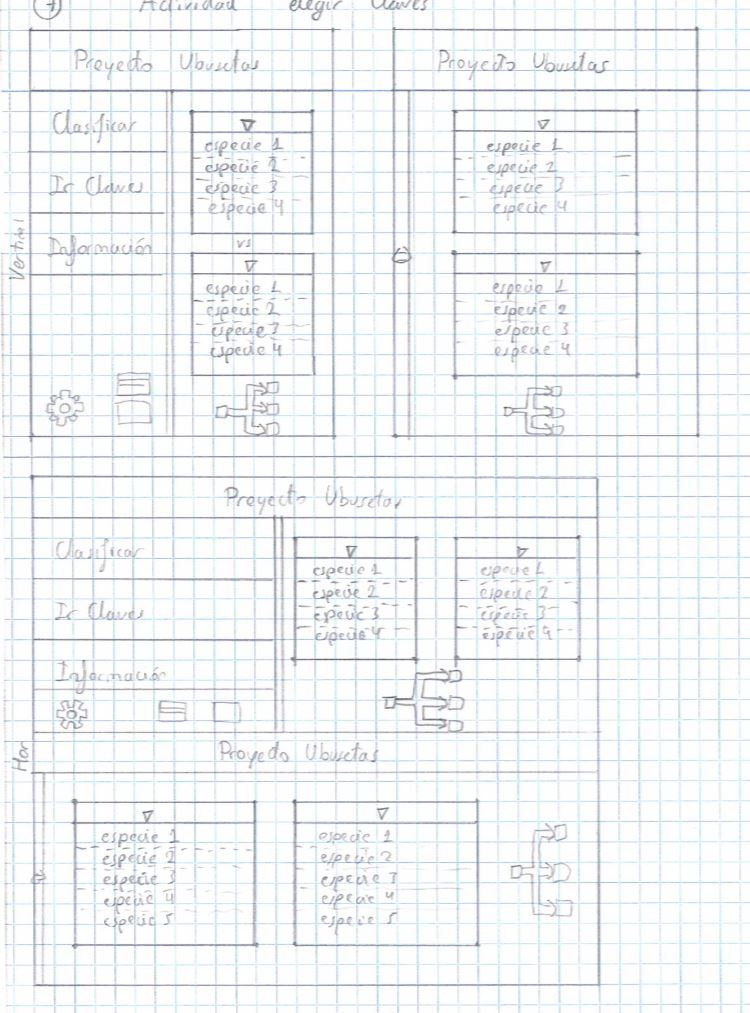
\includegraphics[width=0.8\textwidth]{imagenesAnexos/prototipado/ActividadElegirClaves7}%
          	\caption{Prototipo Elegir Claves.}%
          	\label{figActividadElegirClaves7}%
        	\end{center}%
  		\end{center}%
	\end{figure}%
	\clearpage
	
		%8-ACTIVIDAD MOSTRAR COMPARATIVA
	
	\item Actividad Mostrar Comparativa \ref{figActividadMostrarComparativa8}:
	\begin{figure}[h]
    	\begin{center}%
        	\begin{center}%
          	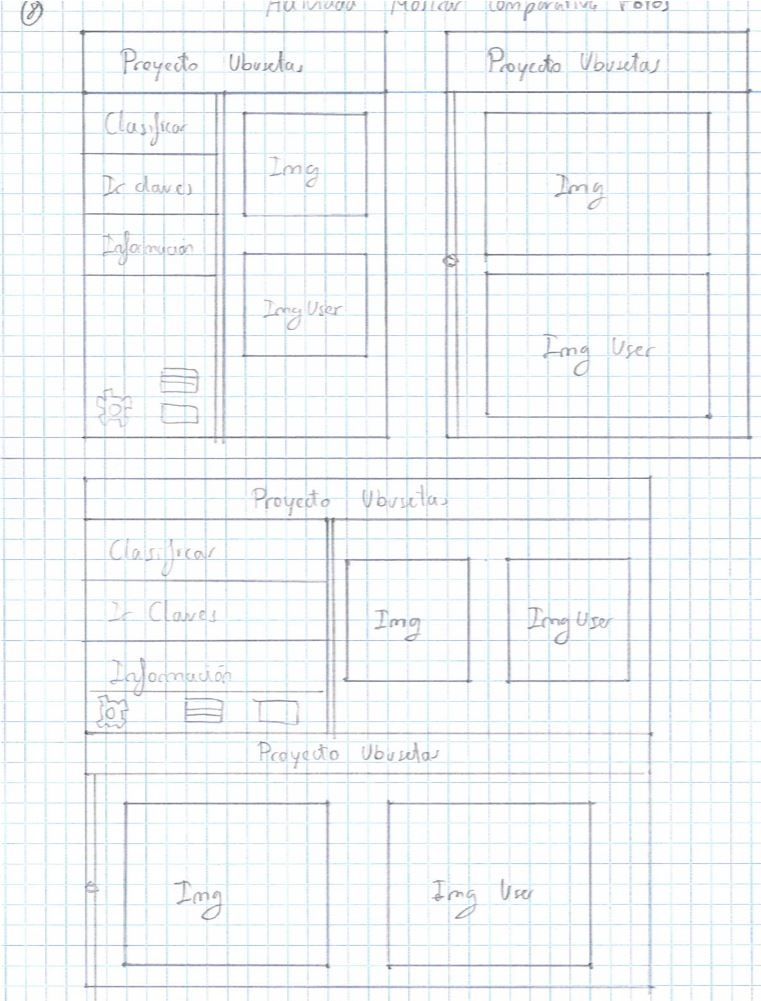
\includegraphics[width=0.8\textwidth]{imagenesAnexos/prototipado/ActividadMostrarComparativa8}%
          	\caption{Prototipo Mostrar Comparativa.}%
          	\label{figActividadMostrarComparativa8}%
        	\end{center}%
  		\end{center}%
	\end{figure}%
	\clearpage
		
		%9-DIAGRAMA DE FLUJO
	
	\item Diagrama de flujo entre las actividades \ref{figDiagramaFlujo}:
	\begin{figure}[h]
    	\begin{center}%
        	\begin{center}%
          	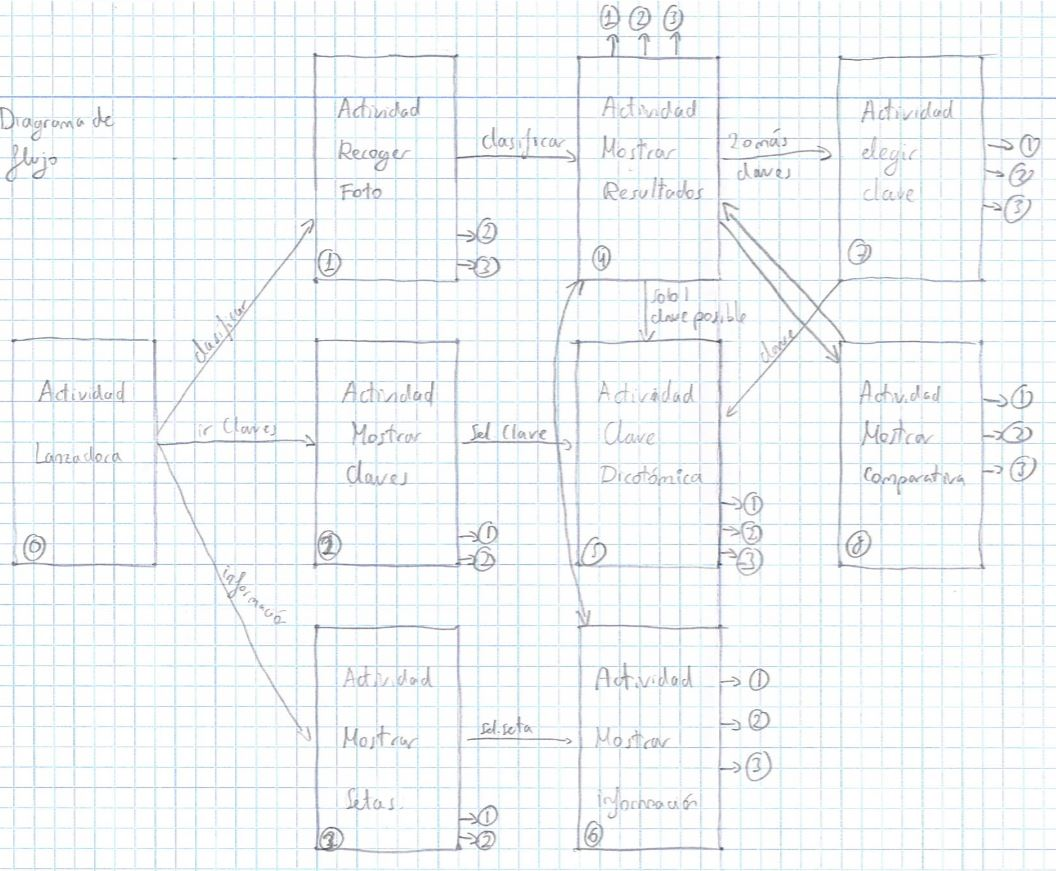
\includegraphics[width=0.8\textwidth]{imagenesAnexos/prototipado/DiagramaFlujo}%
          	\caption{Diagrama de flujo.}%
          	\label{figDiagramaFlujo}%
        	\end{center}%
  		\end{center}%
	\end{figure}%
\end{itemize}

\subsection{Diseño final}

A continuación se muestra un ejemplo del diseño final de la actividad lanzadora en los siguientes estados:
\begin{itemize}
	\item Sin el menú desplegado en vertical \ref{figSinMenu}.
	\item Con el menú desplegado en vertical \ref{figConMenu}.
	\item Sin el menú desplegado en horizontal \ref{figHorizontalSinMenu}.
	\item Con el menú desplegado en horizontal \ref{figHorizontalConMenu}.
\end{itemize}

	\begin{figure}[h]
    	\begin{center}%
        	\begin{center}%
          	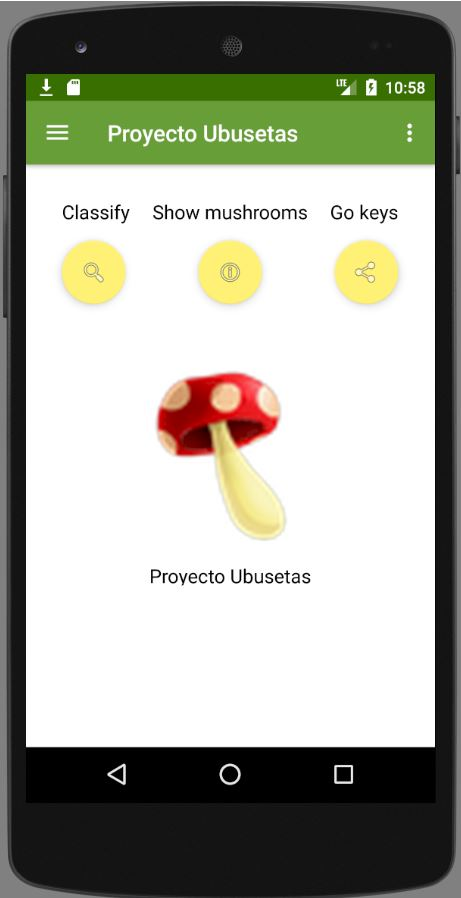
\includegraphics[width=0.8\textwidth]{imagenesAnexos/disenoFinal/SinMenu}%
          	\caption{Vertical sin menú.}%
          	\label{figSinMenu}%
        	\end{center}%
  		\end{center}%
	\end{figure}%
	
	\begin{figure}[h]
    	\begin{center}%
        	\begin{center}%
          	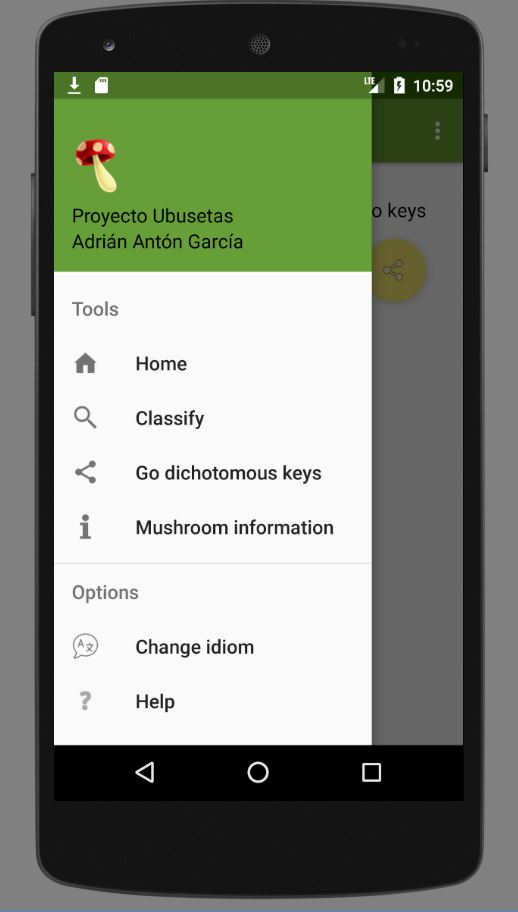
\includegraphics[width=0.8\textwidth]{imagenesAnexos/disenoFinal/ConMenu}%
          	\caption{Vertical con menú.}%
          	\label{figConMenu}%
        	\end{center}%
  		\end{center}%
	\end{figure}%
	
	\begin{figure}[h]
    	\begin{center}%
        	\begin{center}%
          	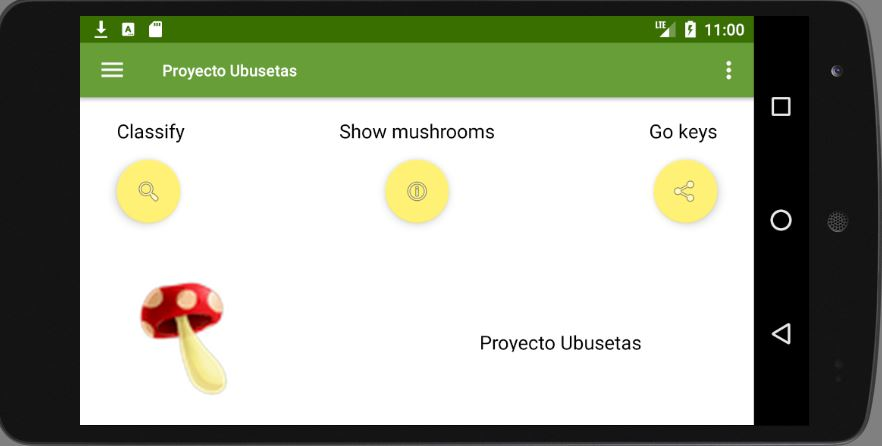
\includegraphics[width=0.8\textwidth]{imagenesAnexos/disenoFinal/HorizontalSinMenu}%
          	\caption{Horizontal sin menú.}%
          	\label{figHorizontalSinMenu}%
        	\end{center}%
  		\end{center}%
	\end{figure}%
	
	\begin{figure}[h]
    	\begin{center}%
        	\begin{center}%
          	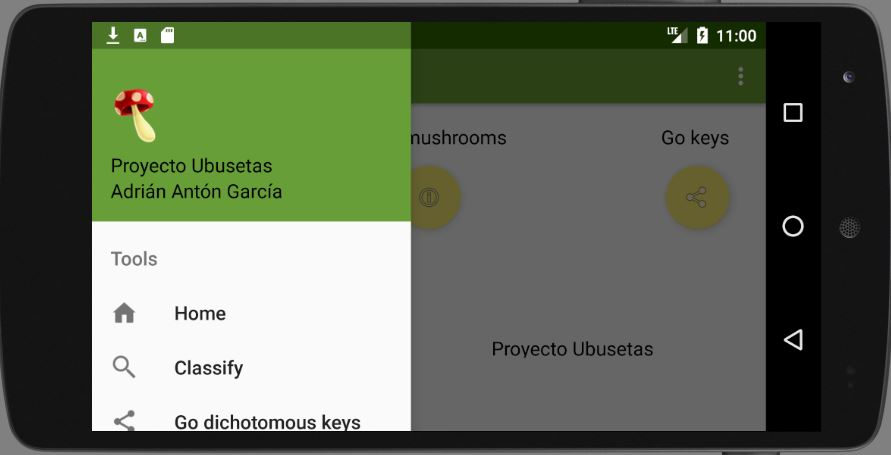
\includegraphics[width=0.8\textwidth]{imagenesAnexos/disenoFinal/HorizontalConMenu}%
          	\caption{Horizontal con menú.}%
          	\label{figHorizontalConMenu}%
        	\end{center}%
  		\end{center}%
	\end{figure}%
\clearpage

\subsubsection{Consideraciones interfaz}

La interfaz se ha desarrollado para adaptarse a múltiples tamaños de pantalla, pero esta opción solo se ha podido probar con unos pocos modelos de móviles por lo que es probable que falle para alguna resolución en concreto.

La aplicación ha sido diseñada para funcionar tanto en modo apaisado como en vertical. Se han intentando seguir las directrices de \textit{Material Design} en cuanto al diseño.